% ArduPilot Software Development: Comprehensive Guide
% Author: Your Name
% Date: \today

\documentclass[12pt,a4paper]{report}
\usepackage[utf8]{inputenc}
\usepackage{graphicx}
\usepackage{hyperref}
\usepackage{amsmath}
\usepackage{geometry}
\usepackage{listings}
\usepackage{caption}
\usepackage{subcaption}
\usepackage{tikz}
\geometry{margin=1in}

\title{ArduPilot Software Development: Comprehensive Guide}
\author{Your Name}
\date{\today}

\begin{document}

\maketitle

\begin{abstract}
This document provides a comprehensive guide to the development, simulation, and extension of the ArduPilot open-source autopilot platform. It covers environment setup, core software components (DroneKit, MAVProxy, pymavlink, Lua scripting), simulation workflows, and troubleshooting, with a focus on practical implementation and extensibility for UAV research and development.
\end{abstract}

\tableofcontents
\listoffigures
\listoftables

% ----------------------
% 1. Introduction
% ----------------------
\chapter{Introduction}
\section{Background}
Unmanned Aerial Vehicles (UAVs), commonly known as drones, have revolutionized fields such as aerial photography, surveying, mapping, and delivery services. The need for reliable, flexible, and open-source autopilot solutions has led to the development of platforms like ArduPilot, which supports a wide range of vehicles including multicopters, planes, and rovers. ArduPilot is widely adopted in both research and industry due to its robust feature set and active community support.

\section{Project Objectives}
The objective of this project is to provide a comprehensive development and simulation environment for ArduPilot, enabling users to:
\begin{itemize}
    \item Develop and test custom drone missions and behaviors.
    \item Interface with ArduPilot using DroneKit, MAVProxy, pymavlink, and Lua scripting.
    \item Simulate missions and analyze results in a controlled environment.
    \item Extend ArduPilot functionalities for research and prototyping.
\end{itemize}

\section{Scope}
This documentation covers the setup, usage, and extension of ArduPilot with supporting tools, focusing on a Windows-based development environment. It is intended for developers, researchers, and hobbyists interested in UAV software development and simulation.

\section{Document Structure}
This document is organized as follows:
\begin{itemize}
    \item Chapter 2 provides a system overview and architecture.
    \item Chapter 3 details the environment setup and directory structure.
    \item Chapter 4 explains the core software components: DroneKit, MAVProxy, pymavlink, and Lua scripting.
    \item Chapter 5 covers simulation and testing workflows, including analysis of results and screenshots.
    \item Chapter 6 presents system diagrams and data flows.
    \item Chapter 7 offers troubleshooting tips and frequently asked questions.
    \item Chapter 8 lists references and further reading.
    \item The Appendix contains additional scripts, logs, and configuration files.
\end{itemize}

% Next chapters to be filled in sequentially...

% ----------------------
% 1. Project Overview
% ----------------------
\chapter{Project Overview}
\section{Introduction}
\section{Project Goals}
\section{System Requirements}
\section{Software Stack}

% ----------------------
% 2. System Overview
% ----------------------
\chapter{System Overview}

\section{What is ArduPilot?}
ArduPilot is an open-source autopilot software suite that supports a wide variety of vehicles, including multicopters, traditional helicopters, fixed-wing aircraft, rovers, boats, and submarines. It provides advanced features such as autonomous mission planning, real-time telemetry, geofencing, fail-safes, and support for a wide range of sensors and hardware platforms. ArduPilot is widely used in both research and industry due to its flexibility, extensibility, and active developer community.

Key features of ArduPilot include:
\begin{itemize}
    \item Support for multiple vehicle types (multicopter, plane, rover, etc.)
    \item Autonomous mission planning and execution
    \item Real-time telemetry and data logging
    \item Integration with ground control stations (GCS) and simulation environments
    \item Extensible via scripting (Lua) and APIs (DroneKit, MAVProxy, pymavlink)
\end{itemize}

\section{Project Architecture}
The project architecture integrates ArduPilot with several supporting tools to enable development, simulation, and mission control. The main components are:
\begin{itemize}
    \item \textbf{ArduPilot Firmware}: The core autopilot software running on the simulated or real vehicle.
    \item \textbf{Simulator (SITL)}: Software-In-The-Loop simulation allows ArduPilot to run on a PC, simulating vehicle dynamics and sensor data.
    \item \textbf{MAVProxy}: A command-line ground control station and middleware that facilitates communication between ArduPilot and other tools.
    \item \textbf{DroneKit}: A Python API for high-level mission scripting and vehicle control.
    \item \textbf{pymavlink}: A Python library for low-level MAVLink protocol communication.
    \item \textbf{Lua Scripting}: Embedded scripting for custom onboard behaviors.
\end{itemize}

\begin{figure}[h!]
    \centering
    \begin{tikzpicture}[node distance=2.5cm]
        \node (user) [draw, rectangle] {User / Developer};
        \node (dronekit) [draw, rectangle, below left=of user] {DroneKit};
        \node (mavproxy) [draw, rectangle, below=of user] {MAVProxy};
        \node (pymavlink) [draw, rectangle, below right=of user] {pymavlink};
        \node (ardupilot) [draw, rectangle, below=of mavproxy, yshift=-1cm] {ArduPilot (SITL)};
        \node (lua) [draw, rectangle, right=of ardupilot, xshift=2cm] {Lua Scripts};
        \node (sim) [draw, rectangle, below=of ardupilot, yshift=-1cm] {Simulator / Vehicle Model};
        \draw[->] (user) -- (dronekit);
        \draw[->] (user) -- (mavproxy);
        \draw[->] (user) -- (pymavlink);
        \draw[->] (dronekit) -- (mavproxy);
        \draw[->] (pymavlink) -- (mavproxy);
        \draw[->] (mavproxy) -- (ardupilot);
        \draw[->] (ardupilot) -- (lua);
        \draw[->] (ardupilot) -- (sim);
    \end{tikzpicture}
    \caption{Project Architecture: Integration of ArduPilot with supporting tools for development and simulation.}
    \label{fig:project_architecture}
\end{figure}

\section{Software Stack}
The software stack for this project consists of the following layers:
\begin{itemize}
    \item \textbf{Operating System}: Windows 10 or later
    \item \textbf{Python Environment}: Python 3.10+ for scripting and API usage
    \item \textbf{ArduPilot SITL}: Software-In-The-Loop simulation of the ArduPilot firmware
    \item \textbf{MAVProxy}: Middleware and command-line ground control station
    \item \textbf{DroneKit}: High-level mission scripting API
    \item \textbf{pymavlink}: MAVLink protocol library for Python
    \item \textbf{Lua}: Embedded scripting for onboard automation
    \item \textbf{Simulation Tools}: Map and mission planning utilities, visualization tools
\end{itemize}

% Next: Environment Setup

% ----------------------
% 3. Environment Setup
% ----------------------
\chapter{Environment Setup}

\section{Hardware and Software Requirements}
To develop and simulate with ArduPilot, ensure your system meets the following requirements:

\subsection*{Hardware}
\begin{itemize}
    \item PC with at least 8 GB RAM (16 GB recommended)
    \item Multi-core processor (Intel i5/i7 or AMD equivalent)
    \item 10 GB free disk space
    \item Internet connection for downloading dependencies and map data
\end{itemize}

\subsection*{Software}
\begin{itemize}
    \item Windows 10 or later (64-bit)
    \item Python 3.10 or newer
    \item Git for Windows
    \item Microsoft Visual C++ Build Tools (for compiling dependencies)
    \item Required Python packages (see requirements.txt)
    \item Optional: Mission Planner or QGroundControl for GUI-based mission planning
\end{itemize}

\section{Installation Steps}
\subsection*{1. Install Python}
Download and install Python 3.10+ from the official website: \url{https://www.python.org/downloads/}. Ensure you add Python to your system PATH during installation.

\subsection*{2. Install Git}
Download and install Git for Windows: \url{https://git-scm.com/download/win}

\subsection*{3. Clone the Project Repository}
Open a terminal (PowerShell or Command Prompt) and run:
\begin{lstlisting}[language=bash]
git clone https://github.com/mustafa-gokce/ardupilot-software-development.git
\end{lstlisting}

\subsection*{4. Install Required Python Packages}
Navigate to the project directory and install dependencies:
\begin{lstlisting}[language=bash]
cd ardupilot-software-development
pip install -r requirements.txt
\end{lstlisting}

\subsection*{5. Install Additional Tools}
\begin{itemize}
    \item Download and install Mission Planner (optional): \url{https://ardupilot.org/planner/docs/mission-planner-installation.html}
    \item Download and install MAVProxy: \url{https://ardupilot.github.io/MAVProxy/html/getting_started/download_and_installation.html}
\end{itemize}

\subsection*{6. Verify Installation}
Test your setup by running a sample script or launching MAVProxy:
\begin{lstlisting}[language=bash]
pip show dronekit
mavproxy.exe --version
\end{lstlisting}

\section{Directory Structure}
The project directory is organized as follows:

\begin{verbatim}
ardupilot-software-development/
├── course-documents/
│   ├── disclaimer.md
│   ├── README.md
│   └── source-codes.md
├── dronekit/
│   ├── dronekit_python310_compat.py
│   ├── ...
├── environment-setup/
│   ├── build-environment-setup.md
│   ├── ...
├── lua/
│   ├── arm_disarm.lua
│   ├── ...
├── mavproxy/
│   ├── arm-disarm.md
│   ├── ...
├── pymavlink/
│   ├── arm-disarm.py
│   ├── ...
├── README.md
├── requirements.txt
\end{verbatim}

\section{Configuration}
After installation, you may need to configure environment variables or tool-specific settings. Refer to the \texttt{environment-setup/} folder for detailed guides on simulation software setup, quickstart scripts, and troubleshooting common setup issues.

% Next: Core Components

% ----------------------
% 4. DroneKit
% ----------------------
\chapter{DroneKit}
\section{Overview}
\section{Example Scripts}
\section{Code Explanations}

% ----------------------
% 5. MAVProxy
% ----------------------
\chapter{MAVProxy}
\section{Overview}
\section{Modules and Commands}
\section{Example Usage}

% ----------------------
% 6. pymavlink
% ----------------------
\chapter{pymavlink}
\section{Overview}
\section{Example Scripts}
\section{Code Explanations}

% ----------------------
% 7. Lua Scripting
% ----------------------
\chapter{Lua Scripting}
\section{Overview}
\section{Example Scripts}
\section{Code Explanations}

% ----------------------
% 8. Simulation and Testing
% ----------------------
\chapter{Simulation and Testing}
\section{Simulation Overview}
\section{Running Simulations}
\section{Simulation Screenshots}
% Example image inclusion:
\begin{figure}[h!]
    \centering
    \includegraphics[width=0.9\textwidth]{images/simulation1.jpg}
    \caption{Simulation: Drone mission path and map overlay.}
    \label{fig:sim1}
\end{figure}

\begin{figure}[h!]
    \centering
    \includegraphics[width=0.9\textwidth]{images/simulation2.jpg}
    \caption{Simulation: Mission progress and telemetry.}
    \label{fig:sim2}
\end{figure}

\section{Analysis of Results}

% ----------------------
% 9. Diagrams
% ----------------------
\chapter{Diagrams}
\section{System Architecture}
\begin{figure}[h!]
    \centering
    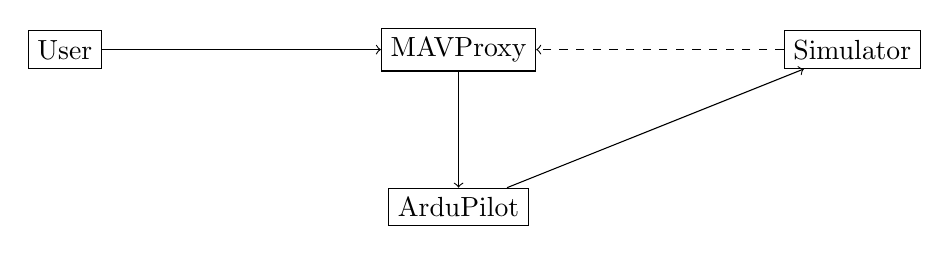
\begin{tikzpicture}[node distance=2cm]
        \node (user) [draw, rectangle] {User};
        \node (mavproxy) [draw, rectangle, right of=user, xshift=3cm] {MAVProxy};
        \node (ardupilot) [draw, rectangle, below of=mavproxy] {ArduPilot};
        \node (sim) [draw, rectangle, right of=mavproxy, xshift=3cm] {Simulator};
        \draw[->] (user) -- (mavproxy);
        \draw[->] (mavproxy) -- (ardupilot);
        \draw[->] (ardupilot) -- (sim);
        \draw[->, dashed] (sim) -- (mavproxy);
    \end{tikzpicture}
    \caption{System Architecture: User commands flow through MAVProxy to ArduPilot and the simulator.}
    \label{fig:arch}
\end{figure}

\section{Data Flow}
\section{Mission Flow}

% ----------------------
% 10. Troubleshooting and FAQs
% ----------------------
\chapter{Troubleshooting and FAQs}
\section{Common Issues}
\section{Solutions}
\section{Frequently Asked Questions}

% ----------------------
% 11. References
% ----------------------
\chapter{References}
% Add your references here

% ----------------------
% 12. Appendix
% ----------------------
\chapter{Appendix}
\section{Additional Scripts}
\section{Logs}
\section{Configuration Files}

\end{document} 